\subsection{统计自然语言处理}



\subsubsection{概率图模型}
将联合概率分布以图的形式来表示, 可以分为有向概率图模型和无向概率图模型. 
概率图模型中, 将随机变量表示为结点, 相关联的随机变量之间会有边连接. 

有向图模型中按变量的因果关系进行连接, 可以刻画变量之间的因果关系. 有向图表示的联合概率可以根据图中的变量依赖关系分解成多个条件概率的积. (听着有点像拓扑图)

无向图模型没有体现出因果关系, 强调的是变量之间的相互关系. 无向图模型将联合概率分布分解为“无向图中-最大团上-随机变量的函数-的乘积”. 





\subsubsection{词袋模型}
用于表示文档/句子(其实句子可以看作只有一个句子的文档)的一种方法. 
词袋模型一般会先构建一个词表, 每个文档经过分词后, 可以使用不同的统计量来构建文档/句子的向量, 词表之外的词不予考虑. 可以选用的不同的统计量有: 
\begin{itemize}
	\item 词频
	\item 布尔词频
	\item TF-IDF
	\item 词向量
\end{itemize}

\subsection{使用朴素贝叶斯分类器进行文本分类}
首先, 给定类别数为$c$, 每个文档的特征向量长度为$n$. 

朴素贝叶斯分类器是一个生成式的分类器, 其计算的是$p(Y | X)$, 对于生成模型, 重要的是要学习联合分布$p(X, Y)$, 朴素贝叶斯通过训练数据学习该联合分布: $p(X, Y) = p(Y)p(X|Y)$. 对于给定样本$X^i$, 对其进行分类可形式化为: 
$$
y = \mathop{argmax}_{c_k} p(Y=c_k | X=X^i) = \mathop{argmax}_{c_k} \frac{p(X=X^i | Y=c_k) p(Y=c_k)}{p(X=X^i)}
$$
朴素贝叶斯中假设样本的特征之间是相互独立的, 即$p(X)=p(X_1=x_1, ..., X_n=x_n) = p(X_1=x_1) ... p(X_n=x_n)$. 那么为了得到样本$X^i$的类别, 只需要计算出$p(X=X^i | Y=c_k),  p(Y=c_k), p(X=X^i)$即可. 而对于某一个样本的分类, $p(X^i)$对分类是没有帮助的, 在$Y$取不同类别时是不会变化的, 故可以不计算$p(X^i)$. 那么剩下的需要计算的只有出$p(X=X^i | Y=c_k),  p(Y=c_k)$了. 

$p(Y=c_k)$是很好计算的, 只需要统计训练数据中类别为$c_k$的样本所占的比例即可. 由于特征之间独立的假设, 所以$p(X^i | Y=c_k) = \prod_{j=1}^{n} p(X_{j}^{i}=x_j | Y=c_k)$. 这个概率也只需要从训练数据中统计即可, 统计每个类别下, 特征向量的第$j$维取$x_j$的比例即可. 

关于样本的特征向量: 通常可以采用词袋模型的方法来表示一个文本/句子. 

\subsection{马尔科夫链/隐马尔科夫链}
马尔可夫模型主要用于研究时间序列的分布的, 若已有一个是时间序列: $X_0, X_1, X_2, ..., X_n$, 马尔可夫模型要解决的就是这些随机变量的取值是如何随着时间而变化的、每个随机变量取值的概率 --- 这些随机变量取值的分布. 随机变量的取值可以称为状态. 那么问题就成了: 
$$
P(X_0=s_0, X_1=s_2, ..., X_n=s_m) = ?
$$
或者说, 下一个时刻的随机变量的取值问题: 
$$
P(X_n | X_0=s_0, X_1=s_2, ..., X_{n-1}=s_{m-1}) = ?
$$
为了简化这个问题, 有了马尔科夫假设. 

(1阶)马尔可夫假设: 当前状态的取值只取决于前一个时刻的状态. 即: 
$$
P(X_n | X_0=s_0, X_1=s_2, ..., X_{n-1}=s_{m-1}) = P(X_n | X_{n-1}=s_{m-1})
$$
满足这样性质的一系列随机变量串联在一起就是马尔科夫链了. 

那隐马尔科夫链与马尔科夫链又有什么关系呢?
隐马尔科夫模型描述的是两个时序序列的联合分布: $p( \boldsymbol{X}, \boldsymbol{Y} )$, 其中$\boldsymbol{X}, \boldsymbol{Y}$均为时序序列, 通常称$\boldsymbol{X}$为观测序列, $\boldsymbol{Y}$为状态序列 --- 不可观测序列. 其中观测序列/状态序列均可视为随机变量序列(注意, 同一时刻的观测变量和状态变量并不是独立的), 观测变量序列的取值为可观测值, 状态变量序列的取值为状态值 --- 与马尔可夫模型中的状态含义一致. 隐马尔科夫模型的假设: 
\begin{itemize}
	\item 当前状态变量$\boldsymbol{Y}_t$的取值仅以来与前一个状态变量$\boldsymbol{Y}_{t-1}$的取值有关, 连续多个状态变量的取值则构成隐马尔科夫链
	\item 任意时刻的观测变量$\boldsymbol{X}_t$取值仅依赖于该时刻的状态变量的取值$\boldsymbol{Y}_t$
\end{itemize}

一个隐马尔科夫模型可以表示为: $\lambda = (\boldsymbol{\pi}, \boldsymbol{A}, \boldsymbol{B})$, 含义如下: 
\begin{itemize}
	\item $\boldsymbol{\lambda}$: 初始状态概率向量, 即初始时刻的状态变量$\boldsymbol{Y}_0$取值为各个状态的概率
	\item $\boldsymbol{A}$: 状态转移概率矩阵, 即上一时刻的状态变量取某值时, 当前时刻状态变量取值的概率分布: $p(\boldsymbol{Y}_t=s_j | \boldsymbol{Y}_{t-1}=s_i)$
	\item $\boldsymbol{B}$: 发射概率矩阵, 即当前状态变量取某值时观测变量取某观测值的概率分布: $p(\boldsymbol{X}_t=o_j | \boldsymbol{Y}_t=s_j)$
\end{itemize}

其实, 可以看出马尔可夫模型是隐马尔科夫模型的一个特例 --- 状态变量序列与观测变量序列相同, 状态值即为观测值, 每个状态只对应一个观测值即本身. 

隐马尔可夫模型的三个应用: 
\begin{itemize}
	\item \textbf{样本生成问题}: 给定模型$\lambda = (\boldsymbol{\pi}, \boldsymbol{A}, \boldsymbol{B})$, 生成满足模型约束的样本 --- 观测序列即对应的状态序列
	\item \textbf{模型的训练}: 给定训练数据 --- 观测序列即对应的状态序列, 估计模型参数$\lambda = (\boldsymbol{\pi}, \boldsymbol{A}, \boldsymbol{B})$
	\item \textbf{序列预测}: 已知模型参数$\lambda = (\boldsymbol{\pi}, \boldsymbol{A}, \boldsymbol{B})$, 给定观测序列, 求状态序列
\end{itemize}

怎么解决上述的三个问题呢?

对于样本生成问题, 其实很简单, 指要逐步采样状态, 得到一个状态序列, 在根据每一步的状态取值采样得到观察值, 就可以得到观测序列, 样本生成就完成了. 

对于模型的训练问题, 需要估计的参数为: $(\boldsymbol{\pi}, \boldsymbol{A}, \boldsymbol{B})$, 对于$\boldsymbol{\lambda}$则统计所有的状态序列中, 计算以每个状态为开头的序列的频率即可, 其他两个概率矩阵的训练类比即可. 

对于序列预测问题可以通过维特比算法解决. 给定一个观测序列, 求解最有可能的状态序列. 本质上这是一个搜索问题, 搜索最有可能的状态序列, 使观测序列的似然概率最大. 简要地说一下. 

维特比算法通过动态规划的方法解决这个问题. 假设我们已经有最优的状态路劲, 那么其中一条从起点开始的子路径也是最优的子路径. 因此可以通过维护两个动态规划的矩阵来记录路径的选择和其概率. 假设有两个矩阵$\boldsymbol{\sigma}, \boldsymbol{\psi}$. 其中$\boldsymbol{\sigma}_{ti}$表示在时刻$t$时以$s_i$结尾的所有局部路径的最大概率, $\boldsymbol{\psi}_{ti}$表示在时刻$t$时末状态为$s_i$的前驱状态. 

\paragraph{应用}使用隐马尔科夫模型可以解中文分词问题. 给定训练数据 --- 每个样本为一个句子, 对于每个样本, 目标是给每个词分配一个标签(如{B, M, E, S}), 然后可以根据序列对句子进行分词. 为达成这个目的, 需要训练隐马尔科夫模型, 获得模型的各个参数, 根据训练数据是否被标注可以使用不同的方法进行训练. 获得训练数据后即可使用模型进行序列预测任务, 再根据序列进行分词. 


\colorbox{red}{注: 本节内容主要参考何晗所著《自然语言处理入门》}. 

\subsection{TF-IDF}
词频-倒排文档频次. 通常用于衡量一个词语在文档中的重要程度. 单单使用词频评价词语重要程度是不全面的, 有些词可能会在文档中出现很多次, 但是如果其在很多文档中都出现, 却又体现不了其重要性. 因此, 需要一个对词频进行扩充, 希望得到的重要的词应该是这样的: 词频高, 同时又不是出现在大部分文档中. 
$$
TF-IDF(t, d) = \frac{TF(t, d)}{DF(t)} = TF(t, d) \cdot IDF(t)
$$
其中, $TF(t, d)$表示词$t$在文档$d$中出现的次数, $DF(t)$表示包含词$t$的文档数. 实际中计算$TF-IDF$时会加入一些平滑操作(如加一平滑、对IDF取对数)防止结果下溢等.  IDF表示inverse document-frequency, 计算方法: 
$$
IDF(t) = \log \frac{1 + n}{1 + DF(t)}
$$
\begin{center}
	或
\end{center}
$$
IDF(t) = \log \frac{n}{1 + DF(t)} + 1
$$
其中 $n$ 是文档数量. 计算得到一个矩阵, 每一行表示一个文档的tf-idf向量, 每个元素表示对应的词(term)在该文档种的重要程度, 一般还会进行$l2$正则化. 

\subsection{Transformer}
在NLP中有很多输入为序列输出为序列的\textbf{seq2seq}任务, 例如机器翻译、文本摘要、序列标注、文本生成等等. 早期的seq2seq任务RNN-based\cite{sutskever2014sequence, cho2014learning}模型为主, 但RNN-based的模型容易出现以下问问题: 
\begin{itemize}
	\item RNN处理seq2seq任务时通常将输入序列转换成一个context向量, 再基于context来得到输出的序列. 单个向量难以包含输入序列的所有信息
	\item RNN在递归的解码过程使得其难以处理长文本序列
	\item RNN的反向传播容易出现梯度弥散/爆炸问题
	\item 序列的处理是串行的, 难以并行化, 计算效率低
\end{itemize}
\textbf{Attention}\cite{bahdanau2016neural, luong2015effective}技术 --- 帮助RNN-based模型解决了一部分困难. 具体是怎么做的呢?在RNN-based模型的基础上主要有以下几个变化: 
\begin{itemize}
	\item 编码器传给解码器的不再只是一个context向量, 会利用编码过程中的所有隐向量
	\item 解码时, 会根据所处的时间步, 为每一个隐向量计算一个分数, 归一化后再分别与隐向量相乘得到当前时间步的context向量
\end{itemize}

有了Attention, RNN-based模型的一部分缺点得到了解决(处理长文本序列的问题), 但还是有一些问题: 不能并行化处理输入序列, 且能不能直接在Attention上构建seq2seq模型呢?

\textbf{Transformer}\cite{vaswani2017attention}来了!!!
Transformer采用的也是编解码的结构: 先对输入序列进行编码, 再根据编码的输出进行解码. 与RNN-based模型不同的是, 其不是递归的处理输入, Transformer可以并行地处理整个文本序列.  

Transformer的模型结构如Fig.\ref{fig:transformer}所示. 具体的计算过程可以参考论文\cite{bivaswani2017attentionbid}的论文笔记. 
\begin{figure}[h] 
	\centering
	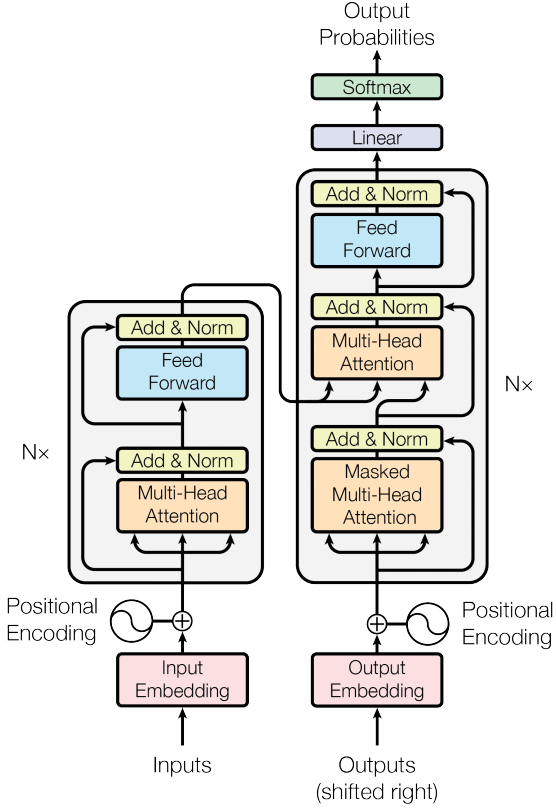
\includegraphics[width=.4\textwidth]{pics/Transformer.png}
	\caption{Architecture of Transformer}
	\label{fig:transformer}
\end{figure}

\begin{itemize}
	\item 由于Transformer没有循环结构, 但是加入了Positional Encoding
	\item 编码部分最终的输出. 会作为Decoder Block中Attention的$K, V$, 解码器的输入作为$Q$
	\item Decoder Block中的Masked Multi-head Attention, 处理当前输入时只允许看到当前位置之前的输入
	\item 在编码器中, 也有mask. 因为通常对输入进行padding
\end{itemize}

\subsubsection{一些关于Transformer的问题}
\paragraph{1.}{\textbf{为什么输入$X$要经过变换得到$Q, K, V$? 为什么不直接使用$X$?}}

如果直接使用$X$, 则$X$直接承担了三种角色: 查询、键和值. 难以学习到满足要求的$X$. 经过变换后得到的$Q, K, V$, $Q$负责表示查询的问题, $V$表示输入的信息, $K$表示与输入相关的“关键词”, $Q, K$相乘用于衡量查询的问题与各条信息之间的相似性. 

\subsection{BERT}
\begin{figure}[h] 
	\centering
	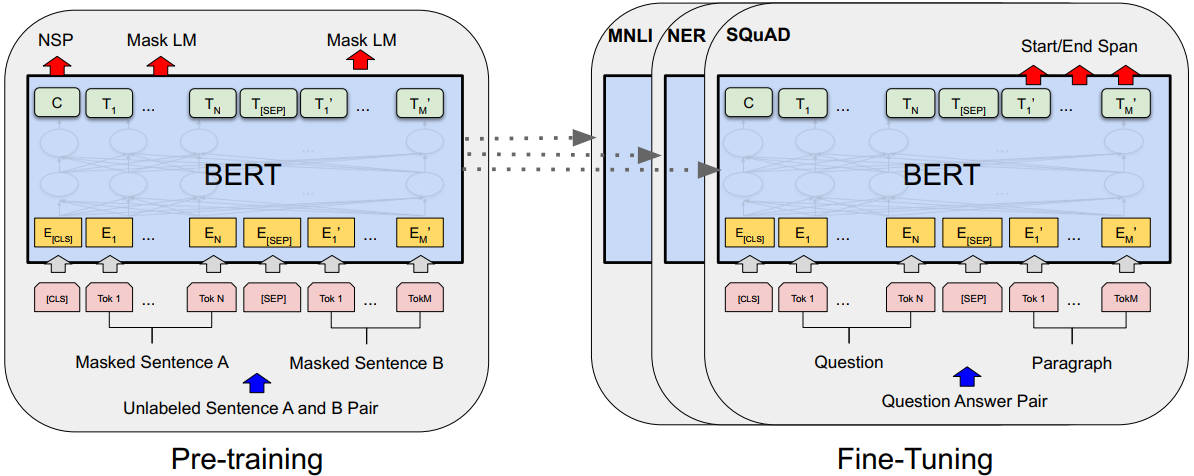
\includegraphics[width=.9\textwidth]{pics/bert-pre training-fine tunning.jpg}
	\caption{Overall pre-training and fine-tuning procedures for BERT}
	\label{fig:bert-pf}
\end{figure}

\paragraph{Motivation}
BERT(Bidirectional Encoder Representations from Transformers)\cite{devlin2019bert}缘自Transformer模型的编码器. 通常的语言模型都是单向的, 例如从左到右, 这使得在处理每个token时只能利用其之前的token. 单向的模型处理token-level的任务时, 难以应用到上下文的信息. 

\paragraph{HOW?}
BERT在大量无标签的文本数据集进行预训练, 得到模型的参数后, 再添加具体任务相关的神经网络层, 微调后即可得到适用于具体任务的模型, 即: pre-training + fine-tuning. 

\par{\textbf{Pre-training}}\ \ \ \ 在预训练阶段, BERT 在大量无标记的的数据上进行训练.  BERT使用两个预训练任务. 
\begin{myitemize}
	\item \textbf{Masked LM}(MLM). 随机 mask 一定比例的输入 tokens, 然后预测这些被 mask 的 tokens. 在最后一层被 mask 的 token 的表征被用于进行预测. 关于 masked tokens 的选择: 随机选择 15\% 的 tokens 被选中, 对于每个被选中的 token, 有 80\% 被替换为 \mintinline{python}{[MASK]}, 有 10\% 被替换为一个随机的 token, 有 10\% 保持不变. \textcolor{red}{为什么要这样做呢?} MLM 的一个负面影响是 pre-training 和 fine-tuning 间的\textbf{不匹配}. 这里的不匹配指的是: \mintinline{python}{[MASK]} 只会在预训练阶段出现, 而不会在微调阶段出现. 若 masked 的 tokens 只用 \mintinline{python}{[MASK]} 表示, 则会使得模型对 \mintinline{python}{[MASK]} 很敏感, 而对其他 token 不敏感. \textbf{计算损失时只在 masked tokens 上进行计算};
	
	\item \textbf{Next Sentence Prediction}(NSP). 这一任务是为了帮助模型理解句子之间的关系. 这一任务是给定两个句子 A, B, 预测 B 是否是 A 的下一个句子. 在这一任务中, 输入的形式是这样的: \mintinline{python}{[CLS] tokens of sentence1 [SEP] tokens of sentence2}. 在最后一层, \mintinline{python}{[CLS]} 的表征被用于进行预测. 这一任务在问答和自然语言推理中都很重要.
\end{myitemize}

\par{\textbf{Fine-tuning}}
预训练结束后就可以用模型来处理下游任务了. BERT 的下游任务的输入有的是单个文本有的是一对文本且输出也可能是不一样的. 针对每个任务, BERT 通过任务特有的输入输出模块来处理. 主要的一些下游任务有: 句子分类(情感分类), token 级别的分类(如词性预测), 两个句子作为输入的预测(例如两个句子之间是否有逻辑关系), 问答任务(例如输入是一篇文章和一个问题, 输出答案在文章中的位置). 

BERT 中\textcolor{red}{可能存在的一些问题}: 1) \mintinline{python}{[MASK]} 在实际预测中并不会出现, 训练时过多的 \mintinline{python}{[MASK]} 会影响模型的表现. 2) 由于每个 batch 中只有 15\% 的数据参与训练, 因此收敛会慢一些.

\begin{figure}[h] 
	\centering
	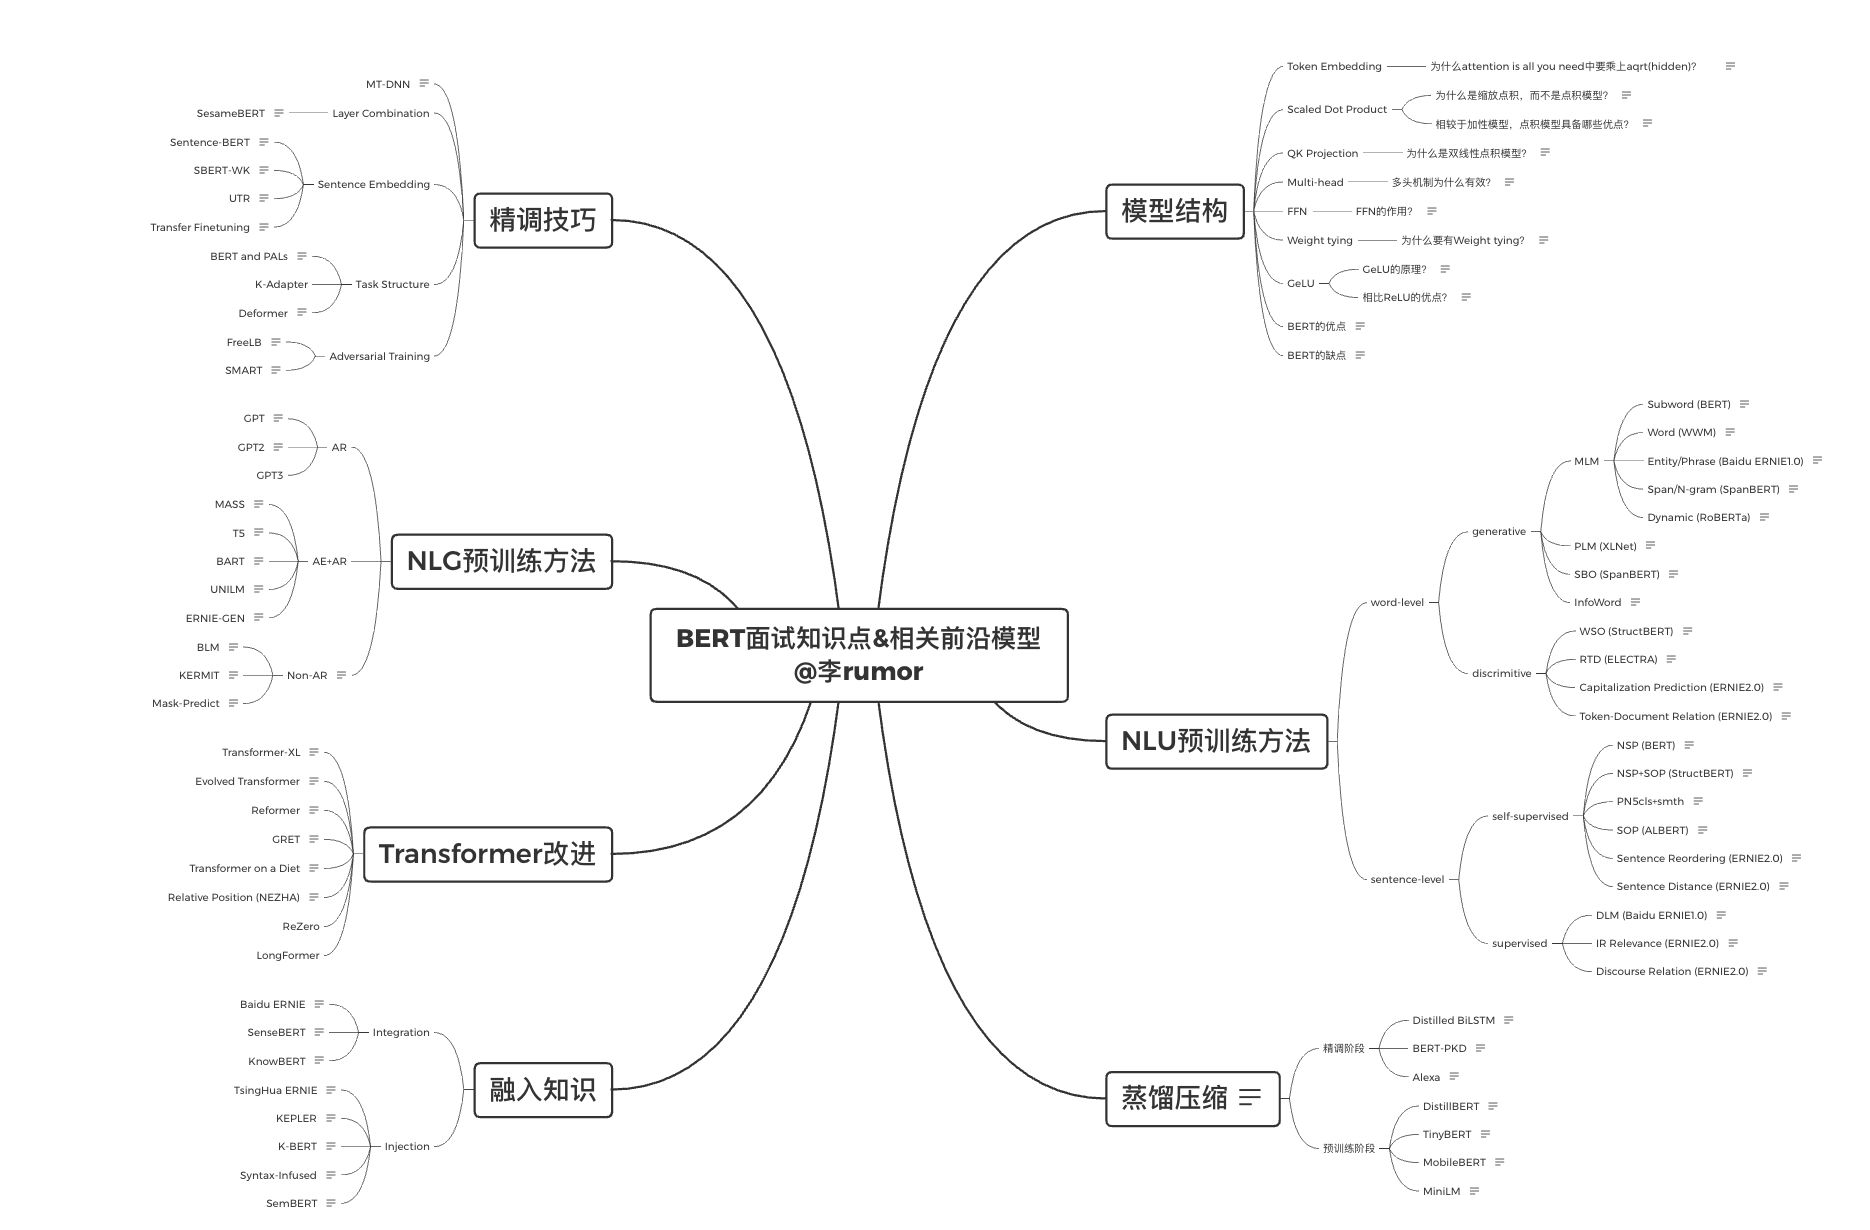
\includegraphics[width=1.1\textwidth]{pics/bert-roadmap.jpg}
	\caption{BERT 知识点总结(\href{https://zhuanlan.zhihu.com/p/46652512}{来源})}
	\label{fig:bert-roadmap}
\end{figure}

参考: \href{https://cloud.tencent.com/developer/article/1666168}{BERT详解(附带ELMo、GPT介绍)}.

\subsection{NeZha}
NeZha\cite{junqiu2019nezha}是华为在预训练模型上的实践总结, 它在BERT的基础上加了很多当下有用的优化, 比如Functional Relative Positional Encoding、Whole Word Masking策略、混合精度训练和LAMB优化器. 实验表明, NeZha在多项具有代表性的中文NLU任务上均取得了不错的成绩. NeZha的模型结构与Bert一致. 
\paragraph{Functional Relative Positional Encoding}有两种对位置进行编码的常用方案: 1)functional PE, 使用正余弦函数来对位置进行编码;2)Parametric PE, 将位置编码作为模型学习的参数. 后续又提出了相对位置编码, NeZha中使用了函数式的相对位置编码. 常用函数是的位置编码: 
$$
\begin{equation}\nonumber
	\left\{\begin{aligned}&\boldsymbol{p}_{k,2i}=\sin\Big(k/10000^{2i/d}\Big)\\ 
		&\boldsymbol{p}_{k, 2i+1}=\cos\Big(k/10000^{2i/d}\Big) 
	\end{aligned}\right.
\end{equation}
$$
其中其中$\boldsymbol{p}_{k,2i}, \boldsymbol{p}_{k,2i+1}$分别是位置$k$的编码向量的第$2i, 2i+1$个分量, $d$是位置向量的维度. 则计算Attention时: 
$$
\begin{equation}\nonumber
	\left\{
	\begin{aligned} 
		\boldsymbol{q}_i =&\, (\boldsymbol{x}_i + \boldsymbol{p}_i)\boldsymbol{W}_Q \\ 
		\boldsymbol{k}_j =&\, (\boldsymbol{x}_j + \boldsymbol{p}_j)\boldsymbol{W}_K \\ 
		\boldsymbol{v}_j =&\, (\boldsymbol{x}_j + \boldsymbol{p}_j)\boldsymbol{W}_V \\ 
		a_{ij} =&\, \frac{e^{ij}}{\sum_k e^{ik}}\\ 
		e_{ij} =& \frac{\boldsymbol{q}_i \boldsymbol{k}_j^T}{\sqrt{d}}\\
		\boldsymbol{o}_i =&\, \sum_j a_{i,j}\boldsymbol{v}_j 
	\end{aligned}\right.
\end{equation}
$$

引入相对位置编码后, 去掉原来的绝对位置编码$\boldsymbol{p}_k$, 分别引入相对位置的$key, value$编码$\boldsymbol{R}_{ij}^K, \boldsymbol{R}_{ij}^V$, 其中$i, j$分别表示序列中元素的位置. 则$\boldsymbol{q}_i$不变, $\boldsymbol{k}_i, \boldsymbol{v}_i$改变, 新的公式如下: 
$$
\begin{equation}\nonumber
	\left\{
	\begin{aligned} 
		\boldsymbol{q}_i =&\, \boldsymbol{x}_i \boldsymbol{W}_Q \\ 
		\boldsymbol{k}_j =&\, \boldsymbol{x}_j \boldsymbol{W}_K + \boldsymbol{R}_{ij}^K \\ 
		\boldsymbol{v}_j =&\, \boldsymbol{x}_j \boldsymbol{W}_V + \boldsymbol{R}_{ij}^V \\ 
		a_{ij} =&\, \frac{e^{ij}}{\sum_k e^{ik}}\\ 
		e_{ij} =& \frac{\boldsymbol{q}_i \boldsymbol{k}_j^T}{\sqrt{d}}\\
		\boldsymbol{o}_i =&\, \sum_j a_{i,j}\boldsymbol{v}_j 
	\end{aligned}\right.
\end{equation}
$$

在一些Parametric relative PE中, $\boldsymbol{R}_{ij}^K, \boldsymbol{R}_{ij}^V$是通过学习得到的, NeZha中通过正余弦函数计算得到: 

\begin{equation}
	\begin{aligned}
		\boldsymbol{R}_{ij}[2 k] =& \sin \left((j-i) /\left(10000^{\frac{2 \cdot k}{d_{z}}}\right)\right) \\
		\boldsymbol{R}_{ij}[2 k+1] =& \cos \left((j-i) /\left(10000^{\frac{2 \cdot k}{d_{z}}}\right)\right)
	\end{aligned}
\end{equation}

NeZha中$\boldsymbol{R}_{ij}^K, \boldsymbol{R}_{ij}^V$是相等的. 

\paragraph{Whole Word Masking}
在BERT中, 是对token进行随机mask的, 但是在中文预料中, 因为通常会进行分词, 所以一个词可能分成了多个token, 若其中一个token被mask, 其他的属于该词的token也应该被mask. mask的概率与BERT一致. 

\paragraph{Mixed Precision Training}
通常模型中的参数和梯度都是保存在32位浮点数. 在NeZha中使用了混合的精度. 在模型的每一次计算过程中, 维护一个32位的权重副本, 然后将其舍入为16位, 再用舍入后的权重进行前向和反向计算, 得到16位的梯度后, 将梯度转为32位, 再用32位的梯度与32位的权重副本来更新权重. 

\paragraph{LAMB Optimizer}
LAMB优化器为大batch-size的训练而生, batch大小可达30000!!!


\subsection{词嵌入模型}
\subsubsection{Word2Vec}

\subsubsection{ELOM}

\subsection{Tokenization}
Tokenizer的目的是: 将文本处理为可以被模型处理的数据. 通常在文本相关的任务中会将文本处理为更细的粒度, 如将篇章处理为句子、句子处理为word、word处理为token, 甚至可以将token处理为character. Tokenizer将文本转化为token, 并基于token表将token转为数字. 常用的tokenization方法: 
\subsubsection{word-based}
一个直接的方法便是以word为token. 通常来说, 可以制定一些规则将文本划分为word序列, 例如英语语料可用空格分割. 但是容易产生以下几个问题: 
\begin{myitemize}
	\item 最终的词汇表可能会非常大
	\item 十分相似的词, 会得到没有关联的id. 如dog和dogs, 被在词汇表中表示为两个词, 但二者的id没有关联, 并不能反映二者真实的语义关系. 这种情况也是使得词汇表庞大的原因之一. 当然, 可以制定规则处理这些情况, 但是还有一些情况难以处理, 如有相同词根的词
	\item 有些词可能会因为时态、词缀等的变化而被视作不同的词, 这也加大了OOV(out of vocabulary)出现的概率	
\end{myitemize}

\subsubsection{character-based}
显然, 这种方法是把原始文本用字符来表示. 这种方式适用于英文, 也适用于中文, 不需要进行分词. 有两个明显的有点: 
\begin{myitemize}
	\item 词汇表会小很多
	\item 出现OOV的概率基本可以消除
\end{myitemize}
但也带了一些很明显的问题: 
\begin{myitemize}
	\item 语义不明显. 将文本分散为character后, 单个character含有的语义太过零散
	\item 处理后的文本包含的token过多, 不利于输入模型, 通常模型的输入是有长度限制的
\end{myitemize}

\subsubsection{subword}
Subword, sub-word, 比我们平常所用的word更小的word, 通常为word的一部分. Subword tokenization的一个原则: 频繁出现的word不应该拆分成sub-word, 而不频繁出现的word应该被分解为更小的、更频繁出现的sub-words. 这种方式可以将较长的word、少见的word分解为常用的sub-words, 且sub-word可以被不同的word之间共享. 


\subsection{BIM}
binary independence model, 二元独立模型. BIM 是一种计算查询与文档相关性的方法. 这种方法通常用在搜索的文档列表排序中, 依据相关性进行排序. BIM 有两个基本假设: 
\begin{itemize}
	\item \textbf{二元假设}: 类似于布尔模型中的文档表示方法, 一篇文档在由特征 (或者单词) 进行表示的时候, 以特征 (或者单词) 出现和不出现两种情况来表示, 不考虑词频等其他因素;
	
	\item \textbf{词汇独立性假设}: 指文档里出现的单词之间没有任何关联, 任意一个单词在文档的分布概率不依赖于其他单词是否出现. 因为词汇之间没有关联, 所以可以将文档概率转换为单词概率的乘积.
\end{itemize} 

\subsubsection{概率检索模型}
一种直接对用户需求进行相关性建模的方法. 对于用户给出的 \textit{query}, 将所有文档分为两类: 相关文档和不相关文档 (\textcolor{red}{如何划分为相关与不相关}). 对于文档 $D$ 来说, $P(R|D)$ 表示文档相关的概率, $P(NR|D)$ 表示文档不相关的概率. 相关性的目标是判断 $P(R|D) > P(NR|D)$ 是否成立. 根据贝叶斯公式转化可得: $\frac{P(D \mid R)}{P(D \mid N R)}>\frac{P(N R)}{P(R)}$. $P(D|R)$, $P(D|NR)$ 表示在相关/不相关文档中观察到 $D$ 的概率. 在排序时并不需要真的分类, 只需要保证相关性由低到高排序即可, 即按照 $\frac{P(D \mid R)}{P(D \mid N R)}$ 降序排序.

\subsubsection{BIM 的推导}
BIM 计算主要集中在上述的两个因子: $P(D|R)$ 和 $P(D|NR)$ 的计算.

根据 BIM 的二元假设, 文档 $D$ 可以表示为一个 0/1 向量, 假设 $D = \{1, 0, 1, 0, 1\}$, 1 表示对应的词出现在 $D$ 中. 用 $p_i$ 表示词汇表中第 $i$ 个单词在相关文档中出现的概率, \textbf{则在已知相关文档集合的情况下}, 观察到 $D$ 的概率为:
$$
P(D|R) = p_1 \times (1-p_2) \times p_3 \times (1-p_4) \times p_5
$$

用 $s_i$ 表示第 $i$ 个单词出现在不相关文档中的概率, 则在不相关文档中观察到 $D$ 的概率为:
$$
P(NR|D) = s_1 \times (1-s_2) \times s_3 \times (1-s_4) \times s_5
$$

\textbf{注意}: $p_i, s_i$ 表示的是第 $i$ 个词在相关 / 不相关文档中出现的概率, 很显然\textbf{在已知相关 / 不相关文档的情况下}, $p_i$可以通过计算在相关文档中有多少文档包含了第 $i$ 个词来计算, $s_i$ 同理.

那么, 可以得到
$$
\frac{P(D \mid R)}{P(D \mid N R)}=\frac{p_{1} \times\left(1-p_{2}\right) \times p_{3} \times\left(1-p_{4}\right) \times p_{5}}{s_{1} \times\left(1-s_{2}\right) \times s_{3} \times\left(1-s_{4}\right) \times s_{5}}
$$
对其进行推广后:
$$
\frac{P(D \mid R)}{P(D \mid N R)}=\prod_{i: d_{i}=1} \frac{p_{i}}{s_{i}} \times \prod_{i: d_{i}=0} \frac{1-p_{i}}{1-s_{i}}
$$
其中 $d_i=1$ 表示文档中出现了的单词, $d_i=0$ 没有出现在文档中. 对上式进行变换:
$$
\begin{aligned}
	\frac{P(D \mid R)}{P(D \mid N R)} &=\prod_{i: d_{i}=1} \frac{p_{i}}{s_{i}} \times\left(\prod_{i: d_{i}=1} \frac{1-s_{i}}{1-p_{i}} \times \prod_{i: d_{i}=1} \frac{1-p_{i}}{1-s_{i}}\right) \times \prod_{i: d_{i}=0} \frac{1-p_{i}}{1-s_{i}} \\
	&=\left(\prod_{i: d_{i}=1} \frac{p_{i}}{s_{i}} \times \prod_{i: d_{i}=1} \frac{1-s_{i}}{1-p_{i}}\right) \times\left(\prod_{i: d_{i}=1} \frac{1-p_{i}}{1-s_{i}} \times \prod_{i: d_{i}=0} \frac{1-p_{i}}{1-s_{i}}\right) \\
	&=\prod_{i: d_{i}=1} \frac{p_{i}\left(1-s_{i}\right)}{s_{i}\left(1-p_{i}\right)} \times \prod_{i} \frac{1-p i}{1-s_{i}} \\
	&=\prod_{i: d_{i}=1} \frac{p_{i}\left(1-s_{i}\right)}{s_{i}\left(1-p_{i}\right)}
\end{aligned}
$$
上式中的第三步 $\prod_{i} \frac{1-p i}{1-s_{i}}$ 是一个与文档无关的量, 因此对同一个 \textit{query} (相关/不相文档划分) 来说, 是不影响文档与 \textit{query} 的相关性排序的, 故可以省去. 对上式的结果取 $\log$:
$$
\log \left(\frac{P(D \mid R)}{P(D \mid N R)}\right)=\sum_{i: d_{i}=1} \log \frac{p_{i}\left(1-s_{i}\right)}{s_{i}\left(1-p_{i}\right)}
$$
接下来的重点就是如何估计 $p_i$, $s_i$ 了, 如前文所述, 只需要统计每个词在相关 / 不相关文档集合中出现的频率即可:
$$
\begin{array}{llll} 
	& \text { 相关文档 } & \text { 不相关文档 } & \text { 文档数量 } \\
	\hline d_{i}=1 & r_{i} & n_{i}-r_{i} & n_{i} \\
	d_{i}=0 & R-r_{i} & (N-R)-\left(n_{i}-r_{i}\right) & N-n_{i} \\
	\hline \text { 文档数量 } & R & N-R & N
\end{array}
$$
因此, $p_i = \frac{r_i + 0.5}{R+1}$, $s_i = \frac{(n_i - r_i) + 0.5 }{(N - R) + 1}$, 其中 0.5 是引入了平滑项以避免为 $\log 0$. 那如何在给定 \textit{query} 的情况下利用以上的内容对文档进行排序呢? 如下:
$$
\text{rel(query, D)} = \sum_{q_{i}=d_{i}=1} \log \frac{\left(r_{i}+0.5\right)\left((N-R)-\left(n_{i}-r_{i}\right)+0.5\right)}{\left(n_{i}-r_{i}+0.5\right)\left(R-r_{i}+0.5\right)}
$$
该式表示 \textit{query} 与 $D$ 的相关性, 其物理意义: 对于同时出现在 \textit{query} 和 $D$ 中的词, 累加每个单词对相关性的贡献, 和就是总的相关性, 于是就可以以此来对文档进行排序了. \textbf{\textcolor{red}{在不确定哪些文档是相关的, 哪些文档是不相关的的时候, 可以给公式的估算因子直接赋予固定值, 则该公式将会退化为IDF因子}}. 例如依从最大熵的原理假设 $p_i = 0.5$, 且相关文档与不相关文档相比只占极小部分, 则可得 $\log \frac{p_i (1 - s_i)}{(1 - p_i) s_i} = \log \frac{1 - s_i}{s_i} = \log \frac{N - n_i + 0.5}{n_i + 0.5} \approx IDF_i$. 所以, \textbf{一个比较关键的问题是如何估计 $p_i, s_i$}, 实际中可以通过用户的点击来估计.

BIM 的缺点也很明显: 只考虑了词是否出现, 不考虑词频对相关性的影响, 忽略了文档长度的影响, 且与现在的深度学习模型相比, 容易因为同义但不相同的词而错过相关的文档.

参考的资料: \href{https://www.cnblogs.com/bentuwuying/p/6730891.html}{概率检索模型: BIM+BM25+BM25F}, \href{https://blog.csdn.net/SrdLaplace/article/details/84954920}{基于词相关性的排序算法}.

\subsection{BM25}
Best Match25. BM25 算法实质上是一个用于信息检索中, 对给定查询 (query) 和若干 "相关" 文档 (document) 进行相关性排序打分的排序函数. BM25 算法其\textbf{主要思想}可简述如下: 对 \textit{query} 进行特征提取分解, 生成若干特征项 (词) $q_i$; 然后对于每个搜索结果文档 $D$, 计算每个特征 $q_i$ 与 $D$ 的相关性得分; 最后将 $q_i$ 相对于 $D$ 的相关性得分进行加权求和, 从而得到 \textit{query} 与 $D$ 的相关性得分. 其计算公式:
$$
\operatorname{score}(\text{query}, D)=\sum_{i} W_{i} \cdot R\left(q_{i}, D\right)
$$
其中 $W_i$ 表示 $q_i$ 的权重, $R(q_i, D)$ 是 $q_i$ 与 $D$ 的相关性得分. 接下来就是如何计算 $W_i$ 和 $R(q_i, D)$ 了. 当然, 在实际使用时, 它们的定义或许并不和下面描述的完全一样.

\subsubsection{$W_i$}
一个词的权重可以有很多衡量方式, 一些传统的方法大多是基于统计来计算的, 比较常用的有 Robertson-Sparck Jones IDF:
$$
\operatorname{IDF}\left(q_{i}\right)=\log \frac{N-n\left(q_{i}\right)+0.5}{n\left(q_{i}\right)+0.5}
$$
其中 $n(q_i)$ 是文档集中包含 $q_i$ 的文档的数量. 可以注意到, 这个式子与上一节的 BIM 结尾处举的例子是一样的, 这种情况值得是初始状态我们不知道哪些文档是相关的, 且相关文档的占比通常是极小的. 所以可以认为 BM25 的权重使用的是特殊情况下的 BIM. $W_i$ 有一个问题还需要注意, 当 $n(q_i)$ 超过 $N$ 的一半时, $W_i$ 就变成负的了, 因此实际使用时通常将这种情况下的 $W_i$ 置为 0.


\subsubsection{$R(q_i, D)$}
一些比较朴素的定义: 特征词在文档中的频率. 但是这种方法难以避免文本长度的影响, 即长文本通常会有更高的词频, 类似于推荐中的热门物品. 还有一个问题就是 $R$ 并不应该与词频是线性关系的, 而应该是增长到一定程度就趋于饱和, 这样就不会\textbf{让某个特征词占据支配地位}. 基于以上考虑, BM25 中的 $R$ 定义为:
$$
\begin{aligned}
	R\left(q_{i}, D\right) &=\frac{\left(k_{1}+1\right) \cdot \tilde{t} f\left(q_{i}, D\right)}{k_{1}+\tilde{tf}\left(q_{i}, D\right)} \\
	\tilde{t f}\left(q_{i}, D\right) &=\frac{t f\left(q_{i}, d\right)}{1+b\left(\frac{L_{D}}{L_{\text {avg }}}-1\right)}
\end{aligned}
$$
其中 $tf(q_i, D)$ 表示 $q_i$ 在 $D$ 中的词频, $L_d, L_{avg}$ 分别为 $D$ 的长度和所有文档的平均长度. $k_1, b$ 为参数, 一般取值范围为 $k_1 \in [1.2, 2.0], b=0.75$. 对上式进行化简:
$$
R(q_i, D) = \frac{(k_1+1) tf(q_i, D)}{k_1[(1 - b) + b \frac{L_D}{L_{avg}}] + tf(q_i, D)}
$$
$k_1$ 起着调节特征词与词频尺度的作用, 很显然, 当 $k_1=0$ 时则 $R$ 成了与词频无关的量, $k_1$ 越大则 $R$ 越接近原始的词频.

\subsubsection{特征词在 \textit{query} 中的重要性}
此外, 若 \textit{query} 比较长, 且某些特征词在 \textit{query} 中的频率比较高, 则这些特征词的重要性也应该提高, 但应该其重要性的提高也应与特征词在文档中重要性一样, 其\textbf{增长也是会饱和的}. 因此在 $score$ 中加入这一项:
$$
R(q_i, query) = \frac{(k_3 + 1) \cdot tf(q_i, query)}{k_3 + tf(q_i, query)}
$$
可以看出这和 $R(q_i, D)$ 是很相似的, $k_3$ 与 $k_1$ 的作用类似, 但是 $R(q_i, query)$ 中没有考虑

BM25 的\textbf{缺点}: 显然, BM25 其实就是 \textit{query} 中每个词与文档的相关性的加权求和, 这一过程肯定是损失了一部分信息的, 如 $q_i$ 之间的顺序关系. 

所以, 最终得到:
$$
score(query, D) = \sum_{i} \log \frac{N-n\left(q_{i}\right)+0.5}{n\left(q_{i}\right)+0.5} \cdot \frac{(k_1+1) tf(q_i, D)}{k_1[(1 - b) + b \frac{L_D}{L_{avg}}] + tf(q_i, D)} \cdot \frac{(k_3 + 1) \cdot tf(q_i, query)}{k_3 + tf(q_i, query)}
$$
其实看这个式子有一个问题, 就是\textbf{\textcolor{red}{特征词在 \textit{query} 中的重要性与文档是无关的, 这样对排序还有用吗?}}

BM25 的\textbf{缺点}: BM25 将文档当作一个整体来进行词频统计 (计算 $R$), 但是显然一个文档的不同部分对 $R$ 的贡献是不等的. BM25 的一些变体对此进行了改进, 如 BM25F 在计算 $R$ 时将文档分割成不同的区域来进行加权统计

参考资料: \href{https://www.cnblogs.com/geeks-reign/p/Okapi_BM25.html}{Okapi BM25算法}(很详细), \href{https://www.cnblogs.com/bentuwuying/p/6730891.html}{概率检索模型: BIM+BM25+BM25F}, \href{https://www.cnblogs.com/NaughtyBaby/p/9774836.html}{BM25 调参调研}(探讨了 BM25 中的参数的影响).

\subsection{Word2Vec}
